\chapter{Definiciones y Notación}
\label{ch:defs}

El objetivo de este capítulo es presentar al lector los conceptos y notaciones que se usarán en los capítulos posteriores.

La inclusión de este capítulo se considera además pertinente para evitar cualquier la ambigüedad en las definiciones. Esta ambigüedad es latente en la literatura de topología digital. Por ejemplo, algunos autores incluyen a los elementos dentro de sus vecindades \cite{cornea2007curve}, mientras que otros los dejan fuera \cite{lam1992thinning}.

Este capítulo comprende los casos 2D y 3D en igual medida. Sin embargo, los algoritmos de cálculo del \textit{skeleton} implementados operan sobre imágenes 3D, por lo que en adelante los conceptos 2D se dejarán de lado. Sin embargo, se incluyen no solo por completitud, sino para facilitar la explicación y comprensión de sus contrapartes tridimensionales.

Desde este capítulo en adelante, salvo cuando se indique expresamente algo distinto, la palabra \textit{algoritmo} se usa siempre para referirse a un algoritmo que calcula el \textit{skeleton}.

\section{Estructura de los datos}

Los algoritmos implementados operan sobre imágenes binarias discretas. Esto quiere decir que su entrada y salida son matrices donde cada elemento vale 0 o 1. En adelante, el término \textit{imagen} se usa para referirse a esta representación matricial. En la literatura esta representación es a veces referida como implícita \cite{bloomenthal1997introduction}. 

Lo anterior significa que las figuras son construidas a partir de un muestreo binario. La manera de efectuar este muestreo en la práctica (el proceso llamado \textit{segmentación}, donde se decide si un punto pertenece o no a la figura) está fuera del alcance de esta tesis, pero en el Capítulo \ref{ch:results} se describe la manera como se hace para la aplicación que motiva este trabajo de tesis.

El \textit{objeto} de una imagen es el conjunto de sus elementos que valen 1. El \textit{fondo} es el conjunto de sus elementos que valen 0. El \textit{skeleton} es el objeto de la imagen que un algoritmo produce como salida.

Si una imagen es de dos dimensiones (2D), los elementos que la constituyen se llaman \textit{píxeles}. Cuando es de tres dimensiones (3D), sus elementos se llaman \textit{vóxeles}. Los \textit{píxeles de objeto} son los píxeles que pertenecen al objeto; es decir, que valen 1. Los \textit{píxeles de fondo} son los píxeles que pertenecen al fondo, cuyo valor es 0. Los \textit{vóxeles de objeto} y \textit{vóxeles de fondo} se definen respectivamente de manera análoga. 

\section{Conceptos de conectividad 2D}

\subsection{Relaciones de vecindad}
En una imagen 2D, cada píxel $p$ tiene exactamente 8 vecinos. Estos son los píxeles que rodean a $p$. Interpretando la imagen 2D como una grilla o celosía regular, donde cada píxel es un cuadrado, los vecinos de $p$ son los píxeles que comparten al menos un vértice con $p$. El conjunto de píxeles formado por $p$ y sus 8 vecinos se denomina la \textit{8-vecindad de $p$}. Es denotado $V_{8}(p)$. Además, se dice que $p$ es un \textit{8-vecino} de los demás elementos de $V_{8}(p)$.

Un tipo de adyacencia más estricto considera solo los vecinos de $p$ que comparten una arista (o, equivalentemente, dos vértices) con $p$. Desde un punto de vista matricial, estos son los vecinos de $p$ que están en la misma fila o columna que $p$. Exactamente 4 píxeles satisfacen esta condición. Entonces, se dice que estos píxeles son \textit{4-vecinos} de $p$. Unidos a $p$, forman la \textit{4-vecindad} de $p$, denotada $V_{4}(p)$.

\begin{figure}[ht]\centering
\includegraphics[width=0.66\linewidth]{images/2dneighborhoods}
\caption{Los 2 tipos de vecindades de un píxel $p$: $V_{4}(v)$ y $V_{8}(v)$}
\label{fig:2dneighborhoods}
\end{figure}

Es claro que $V_{4}(p) \subset V_{8}(p)$. Por consiguiente, si dos píxeles son 4-vecinos también son 8-vecinos. Además, todas las relaciones de vecindad son conmutativas. Si $p$ es $n$-vecino de $q$, entonces $q$ es $n$-vecino de $p$.

\subsection{Caminos y conectividad 2D} \label{conn2D}

Un \textit{8-camino} es una sucesión de píxeles $(p_{0}, p_{1}, \ldots, p_{k})$ que satisface dos condiciones. En primer lugar, todos sus píxeles son de objeto. En segundo lugar, cada uno de ellos, salvo el último, es 8-vecino del siguiente. Luego, se dice que dos píxeles $p$ y $q$ están \textit{8-conectados} si existe un 8-camino que empieza en $p$ y termina en $q$.

Análogamente, dos píxeles $p$ y $q$ están \textit{4-conectados} si existe un \textit{4-camino} que empieza en $p$ y termina en $q$.

Estas nociones de conectividad son fáciles de interpretar. Dos píxeles de objeto $p$ y $q$ están 8-conectados si es posible ir desde $p$ hasta $q$ moviéndose solamente entre 8-vecinos de valor 1. De igual modo, $p$ y $q$ están 4-conectados cuando esta secuencia de movimientos es posible sin efectuar movimientos diagonales.

\section{Conceptos de conectividad 3D}

\subsection{Relaciones de vecindad}
Como se señaló anteriormente, una imagen 2D puede ser interpretada como una grilla regular, donde cada píxel es un cuadrado que comparte aristas y vértices con sus vecinos. Extendiendo esta misma noción, en una imagen 3D cada vóxel se puede interpretar como un cubo dentro de una grilla regular tridimensional. Entonces, cualquier vóxel $v$ puede ser ubicado en el centro de una subgrilla de $3\times3\times3$ vóxeles. El conjunto de vóxeles que pertenecen a esta subgrilla se denomina la \textit{26-vecindad de v}, porque en ella 26 vóxeles rodean a $v$. Se denota $V_{26}(v)$ y se dice que $v$ es \textit{26-vecino} de los demás elementos de $V_{26}(v)$. Todos los vóxeles de este conjunto, y solo ellos, comparten al menos un vértice con $v$ dentro de la grilla.

Un subconjunto importante de $V_{26}(v)$ son los vóxeles que comparten una cara con $v$. Como cada cubo de la grilla tiene 6 caras, existen 6 vóxeles con esta característica. El conjunto formado por estos vóxeles y $v$ se denomina la \textit{6-vecindad de v}, y se denota $V_6(v)$. Se dice que $v$ es \textit{6-vecino} de los demás vóxeles de $V_6(v)$.

Existe además un tercer tipo de adyacencia dentro de $V_{26}(v)$: los vóxeles que comparten alguna arista (o, equivalentemente, por lo menos dos vértices) con $v$. Esta condición significa excluir a los vecinos de $v$ que comparten exactamente 1 vértice con $v$. Gráficamente, quedan fuera los 8 vóxeles que ocupan las esquinas de la subgrilla de $3\times3\times3$ centrada en $v$. El conjunto conformado por $v$ y sus 18 vecinos restantes se denomina la \textit{18-vecindad de $v$}. Es denotado $V_{18}(v)$. Se dice que $v$ es \textit{18-vecino} de los demás elementos de este conjunto. 

Es conveniente destacar que $V_{6}(v) \subset V_{18}(v) \subset V_{26}(v)$. Por lo tanto, si dos vóxeles $v$ y $w$ son 6-vecinos, también son 18-vecinos y 26-vecinos.

\begin{figure}[ht]\centering
\includegraphics[width=0.8\linewidth]{images/3dneighborhoods}
\caption{Los 3 tipos de vecindades de un vóxel $v$: $V_{26}(v)$, $V_{6}(v)$ y $V_{18}(v)$}
\label{fig:3dneighborhoods}
\end{figure}

\subsection{Caminos y conectividad 3D}

Al igual que para imágenes 2D, se define un tipo de camino por cada tipo de vecindad en una imagen 3D. Así, en imágenes 3D la definición de camino de la sección \ref{conn2D} se extiende para vóxeles, dando origen a \textit{26-caminos}, \textit{18-caminos} y \textit{6-caminos}.

Se dice que dos vóxeles $v$ y $w$ están \textit{26-conectados} si existe un 26-camino que empieza en $v$ y termina en $w$. De manera análoga, dos vóxeles pueden estar \textit{18-conectados} y \textit{6-conectados}.

\section{Conectividad en imágenes}

\subsection{Componentes conexas}

Dentro de una imagen, una \textit{componente $n$-conexa}, con $n \in \{4, 8\}$ si la imagen es 2D y $n \in \{6, 18, 26\}$ si es 3D, es un conjunto no vacío de píxeles o vóxeles que satisface dos condiciones. En primer lugar, cada elemento del conjunto está $n$-conectado con todos los demás. En segundo lugar, ningún elemento del conjunto está $n$-conectado con algún elemento fuera del conjunto. Es decir que, usando como ejemplo el caso 3D, dado un vóxel $v$, la componente $n$-conexa que contiene a $v$ es el conjunto maximal de vóxeles $n$-conectados a $v$. Si un conjunto no es $n$-conexo, se dice que es \textit{$n$-disconexo}.

\subsection{Condición básica para la preservación topológica} \label{ssec:fakehomotopy}

En la Sección \ref{sec:skelprops} se ha mencionado como requisito fundamental para la correctitud de un algoritmo el que la imagen de salida sea homotópica con la imagen de entrada. En la práctica, esta preservación topológica se traduce en que la imagen de salida debe tener el mismo número de componentes conexas de objeto y de fondo que la imagen de entrada \cite{saha1994topology}. Estos números dependen del tipo de conectividad que se escoja. Por ejemplo, la imagen de la Figura \ref{fig:8connectedcross} tiene 1 componente conexa de objeto y 1 componente conexa de fondo, independientemente de si se verifica la 4-conectividad o la 8-conectividad. Sin embargo, cambiar el valor del píxel marcado a 0 no altera el número de componentes 8-conexas, pero sí el de 4-conexas. Tras el cambio, la imagen quedaría con 4 componentes 4-conexas de objeto y 2 componentes 4-conexas de fondo. Por lo tanto, un algoritmo que cambiara el valor del píxel rojo a 0 cumpliría con la propiedad homotópica si se usa la 8-conectividad y simultáneamente no la cumpliría si se usa la 4-conectividad.

\begin{figure}[ht]\centering
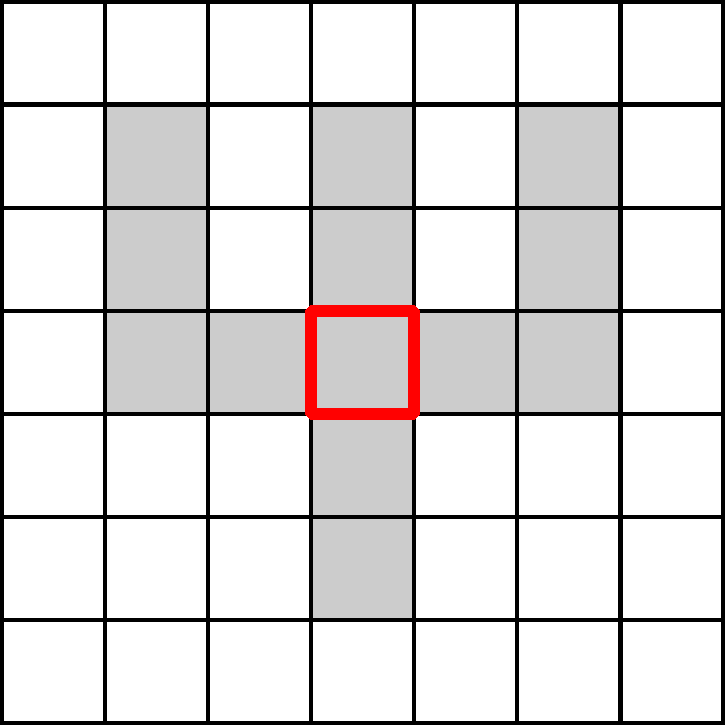
\includegraphics[width=0.35\linewidth]{images/8connectedcrossv2}
\caption{Removiendo el píxel marcado, objeto y fondo se mantienen 8-conexos, pero ambos se vuelven 4-disconexos.}
\label{fig:8connectedcross}
\end{figure}

\subsection{La paradoja del fondo} \label{ssec:paradox}

Casos como el anterior vuelven necesario convenir cuál tipo de conectividad se usará. Una posibilidad sería fijar la 8-conectividad para imágenes 2D y la 26-conectividad para imágenes 3D, argumentando que esto permitiría mayor libertad en la forma del \textit{skeleton}. Así, el \textit{skeleton} podría reproducir la forma del objeto original con mayor fidelidad.

Sin embargo, la Figura \ref{fig:diamong} ilustra una insatisfacción perceptual que resulta de elegir cualquier conectividad, descrita primero en \cite{duda1967graphical}. En esta imagen, tanto fondo como objeto son componentes 8-conexas, cuando la intuición sugiere que el objeto, un \textquotedblleft diamante\textquotedblright{}  8-conexo, debería dividir al fondo en un ``interior'' y un ``exterior''. De examinarse 4-conectividad, el diamante, siendo totalmente 4-disconexo, sí separaría al fondo en 2 componentes 4-conexas. El problema persiste en 3D. Basta pensar en una imagen donde el objeto sea el conjunto $V_{6}(v) - \{v\}$, para algún vóxel $v$ fijo. En esa imagen, tanto objeto como fondo serían 26-conexos, 18-conexos y 6-disconexos a la vez. Sin tratarse de un problema matemático, el que una componente disconexa separe componentes conexas, y viceversa, dificulta la comprensión de la topología digital \cite{rosenfeld1966sequential}.

\begin{figure}[ht]\centering
\includegraphics[width=0.35\linewidth]{images/diamong}
\caption{Imagen donde objeto y fondo son 8-conexos y 4-disconexos al mismo tiempo.}
\label{fig:diamong}
\end{figure}

La ambigüedad desaparece si se escoge algún tipo de conectividad para el objeto y uno diferente para el fondo. Para esta tesis se adopta la convención más común \cite{kong1989digital}. Se usará la 8-conectividad para el objeto y la 4-conectividad para el fondo en imágenes 2D. En imágenes 3D, se usará la 26-conectividad para el objeto y la 6-conectividad para el fondo. Siguiendo esta convención, es posible afirmar que en la Figura \ref{fig:diamong} el diamante conexo efectivamente desconecta al fondo.

\subsection{Búsqueda de componentes conexas}

Recorrer alguna componente conexa es un paso común dentro de los algoritmos implementados en esta tesis. Por lo general no es requisito etiquetar ni contar todas las componentes de una imagen (para lo cual existen algoritmos más apropiados \cite{thurfjell1992new}), sino recorrer alguna componente en particular a partir de un píxel o vóxel determinado. De acuerdo a \cite{vincent1991watersheds}, esto se consigue en tiempo lineal adaptando algún algoritmo de búsqueda en grafos para que recorra elementos de imágenes en lugar de nodos. La elección del algoritmo es arbitraria, porque el orden del recorrido no es relevante.

\begin{algorithm}
\caption{Recorrer una componente conexa por búsqueda en profundidad}
\label{alg:dfscc}
\begin{algorithmic}[1]
\Function{RecorrerCCporBEP}{$I$, $p$, $n$}
	\State\Comment{$I$ es la imagen, $p$ es el píxel o vóxel inicial, $n$ es la conectividad}
	\State $s \gets$ stack()
    \State $s$.push($p$)
    \While {$\neg$ $s$.empty()}
		\State $q \gets$ $s$.pop()
    	\If {$q$ no ha sido marcado como visitado}
    		\State marcar $q$ como visitado\Comment{Por lo general se hace algo con $q$ además de marcarlo}
			\ForAll{$r \in V_{n}(q) - \{q\}$}
            	\If {$val(q) = val(r)$} \label{valfirstuseever} \Comment{$val(x)$ es el valor de $x$ en la imagen, 0 o 1}
                  \State $s$.push($r$)
                \EndIf
    		\EndFor
        \EndIf
  	\EndWhile
\EndFunction
\end{algorithmic}
\end{algorithm}

El Algoritmo \ref{alg:dfscc}, implementado en esta tesis, corresponde a la búsqueda en profundidad \cite{hopcroft1973algorithm} adaptada a imágenes. En él, se comienza por ingresar en una pila todos los $n$-vecinos $n$-conectados a un nodo inicial $p$. Este proceso se repite recursivamente hasta vaciar la pila. La implementación iterativa para la recursión superó en eficiencia al uso de llamadas recursivas. Cabe señalar que la conectividad $n$ se podría inferir a partir del número de dimensiones de la imagen y de si $p$ es de objeto o de fondo, según la convención descrita en la sección anterior. Sin embargo, $n$ se explicita porque en ocasiones se querrá recorrer componentes conexas sin necesariamente obedecer esa convención.

\section{Criterios de preservación topológica}

\subsection{Noción de simplicidad}

Un píxel o vóxel de objeto es \textit{simple} si cambiar su valor a 0 (o \textit{eliminarlo}) no altera la topología de la imagen. Para saber si un elemento es simple, se podría calcular el número de componentes conexas en la imagen antes y después de eliminarlo, usando por ejemplo el Algoritmo \ref{alg:dfscc}, y revertir la eliminación si ese número cambia. Sin embargo, existen métodos más eficientes, capaces de determinar si un elemento es simple revisando nada más que su vecindad. A continuación se describen los métodos implementados para esta tesis.

\subsection{Simplicidad en 2D}

Precisando lo señalado anteriormente, un píxel de objeto es simple si eliminarlo no cambia el número de componentes 8-conexas de objeto ni el número de componentes 4-conexas de fondo. En este sentido, como fue demostrado en \cite{stefanelli1971some}, si un algoritmo elimina solamente píxeles simples efectivamente preserva la topología de la imagen. En otras palabras, un algoritmo que solamente elimine píxeles simples siempre cumplirá con la propiedad homotópica.

\begin{figure}[ht]\centering
\includegraphics[width=0.35\linewidth]{images/2dsimpletestimageextract}
\caption{Numeración de la vecindad de $p$ para construir su grafo de vecindad.}
\label{fig:2dsimplen8}
\end{figure}

El criterio para determinar la simplicidad en imágenes 2D implementado en esta tesis es el que aparece en \cite{siddiqi2002hamilton}. Dado un píxel $p$, se numera su 8-vecindad como se muestra en la Figura \ref{fig:2dsimplen8}. Nótese que $p$ no se numera. El \textit{grafo de vecindad de} $p$ se construye situando primero un nodo sobre cada píxel de objeto numerado y luego una arista entre cada par de nodos situados sobre píxeles 8-vecinos entre sí. Si alguna de las 3-tuplas $(2, 3, 4)$, $(4, 5, 6)$, $(6, 7, 8)$ u $(8, 1, 2)$ corresponde a nodos del grafo, se elimina la respectiva arista diagonal $(2, 4)$, $(4, 6)$, $(6, 8)$ u $(8, 2)$. Con esto se remueven los posibles ciclos de largo 3.

\begin{figure}[ht]\centering
\includegraphics[width=0.6\linewidth]{images/2dsimpletestgraphcases}
\caption{Grafos de vecindad para dos píxeles distintos. En ambos casos la arista que conectaba los nodos 6 y 8 ha sido removida.}
\label{fig:2dsimpleexamples}
\end{figure}

Examinar las relaciones de adyacencia entre los nodos del grafo de vecindad de $p$ indica qué sucedería al eliminar $p$. Si la eliminación de $p$ desconectaría el objeto, el grafo de vecindad de $p$ es disconexo. Si la eliminación de $p$ originaría una componente de fondo (un ``agujero''), el grafo de vecindad de $p$ tiene un ciclo. Un grafo conexo sin ciclos es un árbol. Por lo tanto, se cumple el siguiente lema:

\begin{prop}
Un píxel $p$ es simple si su grafo de vecindad es un árbol.
\end{prop}

Un criterio directo para determinar si el grafo de vecindad es un árbol consiste en comprobar si su característica de Euler, el número de vértices menos el número de aristas, es igual a 1. La Figura \ref{fig:2dsimpleexamples} muestra ejemplos donde $p$ es simple y donde no.

\subsection{Simplicidad en 3D}
\label{ssec:3Dsimplicity}

Además de componentes conexas, las imágenes 3D pueden presentar un elemento topológico adicional. La Figura \ref{fig:tunnelexample} ilustra un ejemplo. Difíciles de definir y encontrar \cite{svensson2003finding}, los  \textit{túneles} también deben considerarse al evaluar la preservación topológica de un algoritmo \cite{cornea2007curve}. Informalmente, un túnel es un agujero que atraviesa un objeto sin desconectarlo. Una definición formal de túnel puede encontrarse en \cite{kong1989digital2}, pero no es necesaria para esta tesis. Solo es preciso considerar que la eliminación de un vóxel puede originar un túnel, alterando con ello la topología de la imagen sin cambiar el número de componentes conexas. Por lo tanto, un algoritmo 3D satisfará la propiedad homotópica si el \textit{skeleton} que calcula preserva el número de componentes 26-conexas de objeto, el número de componentes 6-conexas de fondo y además el número de túneles de la imagen original \cite{Lieutier20041029}.

\begin{figure}[ht]\centering
\includegraphics[width=0.4\linewidth]{images/tunnelexample}
\caption{Ejemplo de imagen 3D con un túnel.}
\label{fig:tunnelexample}
\end{figure}

Se han propuesto varios criterios para determinar la simplicidad de un vóxel \cite{kong1989digital2, tsao1981parallel, university1981three}. En esta tesis se utiliza la caracterización provista por Bertrand y Malandain \cite{bertrand1994new}. Esta caracterización comienza por definir dos números:

\begin{itemize}
\item $C(v)$ como el número de componentes 26-conexas de objeto en $V_{26}(v) - \{v\}$ y
\item $\bar{C}(v)$ como el número de componentes 6-conexas de fondo en $V_{18}(v) - \{v\}$ con algún vóxel 6-vecino a $v$.
\end{itemize}

Luego, se cumple el siguiente teorema:
\begin{theorem}
Un vóxel $v$ es simple ssi $C(v) = 1$ y $\bar{C}(v) = 1$.
\end{theorem}

Tener en cuenta la noción de punto simple al diseñar un algoritmo basta para satisfacer la propiedad homotópica. Como se ha dicho antes, la topología podría conservarse con imponer la restricción de eliminar exclusivamente puntos simples. Sin embargo, esta estrategia no asegura en ninguna medida el resto de las propiedades del \textit{skeleton}. Los píxeles de los extremos de una línea, por ejemplo, son simples, pero eliminarlos significaría perder información de la forma de la figura (es más, la línea podría ser transformada en un punto aplicando sucesivamente este criterio).

\begin{figure}[ht]\centering
\includegraphics[width=0.7\linewidth]{images/voxel_types}
\caption{Principales tipos de vóxeles}
\label{fig:voxeltypes}
\end{figure}

\subsection{Píxeles y vóxeles de término}

Un \textit{píxel de término} es un píxel de objeto que tiene exactamente 1 píxel de objeto 8-vecino. Similarmente, un \textit{vóxel de término} es un vóxel de objeto que tiene exactamente 1 vóxel de objeto 26-vecino.

El que un elemento sea de término significa que está en el extremo de una línea. En principio, todas las líneas son necesarias para que el \textit{skeleton} exprese la forma del objeto original con fidelidad, por lo que un algoritmo debería preservar todos los elementos de término. No obstante, algunas líneas pueden ser poco relevantes, por lo que todo algoritmo debe obedecer algún criterio para decidir si un elemento de término debe ser eliminado. En cuán relajado sea este criterio radica en qué medida el resultado producido por un algoritmo favorecerá la propiedad de reconstructibilidad (en perjuicio de otras propiedades, como la suavidad y la robustez).

\section{Sobre los datos de prueba}

En los capítulos posteriores se usarán algunas imágenes 3D para ilustrar los resultados de cada algoritmo. Estas imágenes fueron obtenidas voxelizando mallas de superficie en formato OFF pertenecientes a la base de datos Princeton Shape Benchmark \cite{shilane2004princeton}. La voxelización se hizo con el programa binvox de Patrick Min \cite{patrick2011binvox}, usando el comando:

\begin{center}
\texttt{binvox -d 128 128 128 <ruta malla original> <ruta archivo de salida>}
\end{center}

Ejecutar este comando produce un archivo de vóxeles en un formato especial para binvox. La especificación y lectura en MATLAB de este formato se detalla en los apéndices. El parámetro \texttt{-d 128 128 128} indica las dimensiones del archivo de vóxeles, es decir, la resolución del muestreo de la malla. Estos valores se escogieron por ser los utilizados para mostrar los resultados en el artículo \cite{arcelli2011distance}, que corresponde al tercer algoritmo implementado. La ruta del archivo de salida es relativa a la ruta de la malla original.

En la Figura \ref{fig:test_models_psb} se enlistan las imágenes de prueba que se usarán a lo largo de esta tesis, junto con su código de identificación en la base de datos Princeton Shape Benchmark.

\begin{figure}[H]\centering
\includegraphics[width=0.8\linewidth]{images/test_models_psb}
\caption{Imágenes de prueba obtenidas voxelizando mallas de la Princeton Shape Benchmark Database}
\label{fig:test_models_psb}
\end{figure}

Adicionalmente, se incluyeron 6 imágenes de la base de datos Aim@Shape en el conjunto de pruebas \cite{saboret2007laurent} que aparecen también en \cite{arcelli2011distance}. Esta base de datos actualmente no se encuentra disponible en internet. Los archivos fueron proporcionados por Gabriella Sanniti di Baja, coautora del algoritmo del Capítulo \ref{ch:arcelli}, en formato VOL. En los apéndices también se incluye la especificación de este formato y su lectura en MATLAB.

\begin{figure}[H]\centering
\includegraphics[width=0.8\linewidth]{images/test_models_aas}
\caption{Imágenes de prueba de la base de datos Aim@Shape}
\label{fig:test_models_aas}
\end{figure}
